%%%%%%%%%%%%%%%%%%%%%%%%%%%%%%%%%%%%%%%%%%%%%%%%%%%%%%%%%%%%%%%%%%%%%%%%%%%%%%%%
%2345678901234567890123456789012345678901234567890123456789012345678901234567890
%        1         2         3         4         5         6         7         8

%\documentclass[letterpaper, 10 pt, conference]{ieeeconf}  % Comment this line out
                                                          % if you need a4paper
\documentclass[a4paper, 10pt, conference]{ieeeconf}      % Use this line for a4
                                                          % paper

\IEEEoverridecommandlockouts                              % This command is only
                                                          % needed if you want to
                                                          % use the \thanks command
\overrideIEEEmargins
% See the \addtolength command later in the file to balance the column lengths
% on the last page of the document



% The following packages can be found on http:\\www.ctan.org
\usepackage{graphicx} % for pdf, bitmapped graphics files
%\usepackage{epsfig} % for postscript graphics files
%\usepackage{mathptmx} % assumes new font selection scheme installed
%\usepackage{times} % assumes new font selection scheme installed
\usepackage{amsmath} % assumes amsmath package installed
\usepackage{amssymb}  % assumes amsmath package installed
\usepackage{subfigure,bm,multirow}
\usepackage{booktabs}
\usepackage[table,svgnames]{xcolor}
\title{\LARGE \bf
Improvements in Lip-Based Video Biometric Performance }
% Using Mid-level Spatiotemporal Features

% \author{ \parbox{3 in}{\centering Huibert Kwakernaak*
%          \thanks{*Use the $\backslash$thanks command to put information here}\\
%          Faculty of Electrical Engineering, Mathematics and Computer Science\\
%          University of Twente\\
%          7500 AE Enschede, The Netherlands\\
%          {\tt\small h.kwakernaak@autsubmit.com}}
%          \hspace*{ 0.5 in}
%          \parbox{3 in}{ \centering Pradeep Misra**
%          \thanks{**The footnote marks may be inserted manually}\\
%         Department of Electrical Engineering \\
%          Wright State University\\
%          Dayton, OH 45435, USA\\
%          {\tt\small pmisra@cs.wright.edu}}
% }

\author{Budhaditya Goswami, Chi Ho Chan, Josef Kittler and Bill Christmas% <-this % stops a space
%\thanks{This work was not supported by any organization}% <-this % stops a space
\thanks{All authors are with the Centre for Vision, Speech and Signal Processing, Faculty of Electronics and Physical Sciences, University of Surrey, Guildford, GU2 7XH, United Kingdom {\tt\small \{b.goswami, c.chan, j.kittler, w.christmas\}@surrey.ac.uk}}%
}

\begin{document}
\maketitle
\thispagestyle{empty}
\pagestyle{empty}
%%%%%%%%%%%%%%%%%%%%%%%%%%%%%%%%%%%%%%%%%%%%%%%%%%%%%%%%%%%%%%%%%%%%%%%%%%%%%%%%
\begin{abstract}
The lip-region can be interpreted as either a genetic or behavioral biometric trait depending on whether static or dynamic information is used. Despite this breadth of possible application as a biometric, lip-based biometric systems are scarcely developed in scientific literature compared to other more popular traits such as face or voice. This is because of the generalized view of the research community about the lack of discriminative power in the lip region. In this paper, we propose a new method of texture representation called Local Ordinal Contrast Pattern (LOCP) for use in the representation of both appearance and dynamics features observed within a given lip-region during speech production. The use of this new feature representation, in conjunction with some standard speaker verification engines based on the nearest neighbour classifier, is shown to drastically improve the performance of the lip-biometric trait compared to the existing state-of-the-art methods. The best, reported state-of-the-art performance was an HTER of 13.35\% for the XM2VTS database. We obtained HTER of less than 1\%. The improvement obtained is remarkable and suggests that there is enough discriminative information in the mouth-region to enable its use as a primary biometric modality as opposed to a ``soft'' biometric trait as has been done in previous research. 
\end{abstract}


%%%%%%%%%%%%%%%%%%%%%%%%%%%%%%%%%%%%%%%%%%%%%%%%%%%%%%%%%%%%%%%%%%%%%%%%%%%%%%%%
\section{INTRODUCTION}
Numerous measurements and signals have been investigated for use in biometric recognition systems. 
Among the most popular measurements are fingerprint, face and voice. 
Lip-region features straddle the area between the face and voice biometric. 

There are various factors that make the use of lip features a compelling biometric. 
Lip-motion can be capture non-intrusively since it is a result of speech.
With the advent of cheap camera sensors for imaging, it is easier than ever before to isolate the lip-region features and use them in combination with other biometric traits to enhance the robustness of multi-modal biometric systems. 
The use of talking face features also naturally increases the robustness of the system with respect to any attempts at faking ``liveness''. 
Since the lip data can be captured at a distance, it represents a passive biometric as it requires no active user participation. 
The challenges of using the lip as a biometric lie in the areas of uniqueness and circumvention. 
The research question is therefore: how do we extract accurate and person-specific information from the lip region at a distance and still maintain a sufficient inter-person variation to intra-person variation ratio for accurate verification? 

The physical attributes of the lip region are affected by the craniomaxillofacial structure of an individual.
Since this structure is a physical manifestation of their DNA, the lip can be considered a genetic biometric.
Human lip movement during speech production occurs due to the flexible mandible. 
The means and forms of lip movement depend upon the language and an individual's pronunciation which is affected by numerous socio-economic factors. 
This manifestation of individual behaviour leads to behavioural dynamics of the lip region which in turn can also be used as a biometric.
Notionally, this is akin to the idea of a ``mouth-signature''. 

In this paper, we demonstrate some remarkable improvements in the performance of lip-based biometric systems. 
These improvements are realised through the use of a novel texture descriptor called Local Ordinal Contrast Patterns (LOCP). 
We use this texture representation within a novel configuration called Windowed Three Orthogonal Planes (WTOP), an extension to an approach called Three Orthogonal Planes (TOP). 
TOP was first proposed in the field of speech or action recognition and segmentation. 
It specifies planar directions along which texture features can be computed enabling the quantisation of dynamic texture and appearance information in the mouth-region. 
The combination of LOCP and WTOP is demonstrated to have excellent performance in extracting identity specific information from within a visual speech signal when used with some simple, text-independent speaker verification systems based on Normalised Correlation(NC) and Chi-squared (X2) histogram matching methods.

A taxonomy of the state-of-the art in lip-based speaker verification is presented in Section~\ref{RelevantWork}. A summary of the current performance characteristics of the field is presented in Table~\ref{PerformanceOfLipBiometrics}. A discussion of the relevant approaches leads to the motivation behind the development of the current, novel feature descriptor. The detailed treatment of the use of LOCP features for dynamic texture description is provided in Section~\ref{OCP}. Section~\ref{WTOP} describes the proposed WTOP configuration. The speaker verification systems used to evaluate this novel descriptor are described in Section~\ref{SpeakerVerificationSystems}. The paper concludes with the experimental evaluation in Section~\ref{ResultsAndEvaluation} and some concluding remarks in Section~\ref{Conclusions}.

\section{Relevant Work}
\label{RelevantWork}
\begin{table*}[htbp!]
\centering
\rowcolors{2}{LightPink}{white}
\begin{tabular}{cccccll}
\toprule
\textbf{System}&\textbf{Lip Feature}&\textbf{Database}&\textbf{Clients}&\multicolumn{2}{c}{\textbf{Performance}} \\
\midrule
Faraj\cite{Faraj06Person}&Lip Dynamic TI&\textbf{XM2VTS}&295&EER&22\\ 
Sanchez\cite{Ramos06Fusion}&Lip Dynamic TD&\textbf{XM2VTS}&295&HTER&\textbf{13.35}\\ 
Gomez\cite{Gomez02Biometric}&Static(lip geometric)&Custom&50&EER&0.015 \\ 
Jourlin\cite{Jourlin97Acoustic}&Static(lip shape)&M2VTS&37&HTER&6.85 \\ 
Samad\cite{Samad07Lower}&Lip Dynamic TI&AMP CMU&10&HTER&0.0 \\ 
Wark\cite{Wark97Person}&Lip Dynamic TI&TULIPS1&96&EER&0.0 \\ 
Wark\cite{Wark97Person}&Static(lip shape)&TULIPS1&96&EER&6.3 \\ 
Wark\cite{Wark97Person}&Static(lip intensity)&TULIPS1&96&EER&0.0 \\ \bottomrule
% \hiderowcolors
\textbf{System}&\textbf{Feature Fusion}&\textbf{Database}&\textbf{Clients}&\multicolumn{2}{c}{\textbf{Performance}} \\
\midrule
% \showrowcolors
Broun\cite{Broun02Automatic}&Static(lip geometric) + Audio &\textbf{XM2VTS}&261&HTER&6.3 \\ 
Faraj\cite{Faraj06Person}&Lip Dynamic TI + Audio &\textbf{XM2VTS}&295&EER&2\\ 
Sanchez\cite{Ramos06Fusion}&Lip Dynamic TD + Face&\textbf{XM2VTS}&295&HTER&4.72 \\ 
Sanchez\cite{Ramos06Fusion}&Lip Dynamic TD + Audio&\textbf{XM2VTS}&295&HTER&\textbf{0.74}\\ 
Sanchez\cite{Ramos06Fusion}&Lip Dynamic TD + Face + Audio&\textbf{XM2VTS}&295&HTER&7.06 \\ 
Abdulla\cite{Abdulla09Lips}&Hybrid(lip shape and lip intensity)&Custom&35&EER&18.0 \\ 
Cetingul\cite{Cetingul06Discriminative}&Hybrid(lip texture and lip motion)&MVGL-AVD&50&EER&5.2 \\ 
Cetingul\cite{Cetingul06Multi}&Static(lip texture)&MVGL-AVD&50&EER&1.7 \\ 
Jourlin\cite{Jourlin97Acoustic}&Static(lip shape) + Audio&M2VTS&37&HTER&0.3 \\ 
\bottomrule
\end{tabular}
\caption{Performance of Lip Biometric Systems for Speaker Verification Showing Lip Performance And Fusion Performance}
\label{PerformanceOfLipBiometrics}
\end{table*}
The use of the lip region as a means of human identification was first proposed through the concept of ``lip-prints'' in the field of forensic anthropology as early as the 20th century by investigators such as Fischer and Locard \cite{Kasprzak90Poss}. 
Lip prints contained information about the individual eccentricities of the lip surface. 
The application of lip prints specifically as a biometric trait was introduced in \cite{Suzuki68Trail}. 
A taxonomy of contemporary relevant work can be based on whether the approach uses static or dynamic information from the lip-region. 
This also enables the incorporation of a hybrid class of methods which attempt to capture both types of information. 

\noindent\textbf{Static Methods}: use features extracted from the lip-region to describe its shape, geometric properties or appearance. Additionally, most of these methods either operate on static images using only single-frame information or on a sequence of speech video on a per-frame basis. Examples of such methods are in  \cite{Chibelushi96Design,Jourlin97Acoustic,Cetingul04Use,Gomez02Biometric,Broun02Automatic,Choras08Human}

\noindent\textbf{Dynamic Methods}: use features related to the changes observed in the mouth-region during speech production. 
These systems can be further segregated into two categories. 
Most deployed biometric systems are based on scenarios with cooperative users speaking fixed string passwords from a small vocabulary. 
These generally employ \textbf{\emph{text-dependent}}(TD) systems \cite{Ramos06Fusion}. 
Such constraints are quite reasonable and can greatly improve the system accuracy. 
However, there are cases when such constraints can be impossible to enforce. 
In situations requiring greater flexibility, systems are required that are able to operate without explicit speaker cooperation and independent of the spoken utterance. 
This mode of operation is referred to as \textbf{\emph{text-independent}}(TI) speaker recognition \cite{Faraj06Person,Faraj06Motion,Samad07Lower}.

\noindent\textbf{Hybrid Methods}: exploit both static and dynamic information by performing either score-level or feature-level fusion. \cite{Auckenthaler99lip,Cetingul06Multi,Cetingul06Discriminative,Tamura04Multi,Abdulla09Lips,Wark97Person}.

\noindent\textbf{State-of-the-art Performance Review}: In order for various speaker verification systems to be compared, a variety of factors need to be considered. 
Commonly, lip-based features are evaluated in terms of the performance improvement they provide through multi-modal fusion with more established biometric traits (e.g. audio and face). 
For the testing of speaker verification systems, there exist only a few databases such as \cite{Messer99Xm2vts} with established verification protocols that enable a fair comparison of systems. 
However, some publications use custom-built datasets and evaluation protocols. 
The disadvantage of using such datasets is that in addition to reducing the comparability of the systems, often the classification task is made easier by skewing the ratio of trait feature dimensions to the number of clients in favor of the systems. 
Table~\ref{PerformanceOfLipBiometrics} provides an overview of the performance of various lip-biometric systems. 
For a more thorough description of the various metrics related to speaker verification, the reader is referred to \cite{Bengio01Evaluation}. 

As shown in Table~\ref{PerformanceOfLipBiometrics}, the most commonly used database and protocol are XM2VTS (used by 3 authors) and Lausanne Protocols respectively. 
The performance obtained using lip features \emph{only} on this database are by \cite{Ramos06Fusion}(Half Total Error Rate (HTER) of 13.35\%). Multi-modal fusion with audio features \cite{Ramos06Fusion} yields HTER of 0.74\%. 
In this paper, we use the XM2VTS to ensure the comparability of our results with these reference benchmarks.
\section{Spatiotemporal Descriptors Using Local Ordinal Contrast Patterns}
\label{OCP}
An ordinal contrast encoding is used to measure the contrast polarity of values between a pixel pair (or average intensities between a region pair) as either brighter than or darker than some reference. 
This polarity is then turned into a result value in a binary decision. 
The ordinal measure is invariant to any monotonic transformation such as image gain, bias or gamma correction \cite{conf/eccv/ZabihW94}. 
The pattern represents the relative difference in the immediate local neighbourhood of a given pixel. 
In computer vision, the absolute information contained within a pixel including intensity, color and texture can vary dramatically under various illumination conditions. 
However, the mutual ordinal relationships between neighbours at the pixel-level or region-level continue to reflect the intrinsic nature of the object and  provide a degree of response stability in the presence of such changes. 

Local Binary Patterns (LBP) \cite{conf/SPIE/pietikaeinenONH94} are an example of ordinal contrast patterns.
LBP offers a powerful and attractive texture descriptor showing excellent results in terms of accuracy and computational complexity in many empirical studies. 
The LBP operator measures the ordinal contrast pairs between a local neighbour value and the reference (centre pixel) value. 
The LBP is obtained by concatenating these binary results and then converting the sequence into the decimal number. 
Recently \cite{conf/icig/Jin04} and \cite{conf/amfg/TanT07} have pointed out that LBP misses the local structure if the reference value is affected by noise. 
In an LBP, the effect of measurement noise could result in a situation where the reference value changes by a single unit. 
This change affects all of the 8 ordinal contrast encodings. 
\cite{conf/amfg/TanT07} have proposed Local Ternary Patterns (LTP), which extend LBP by increasing the feature dimensionality depending on the sign of the centre bit, at the expense of not being invariant to monotonic transformation.
\cite{conf/icig/Jin04} proposed, Improved LBP which performs ordinal contrast measurement with respect to the average of the pixel neighborhood instead of the centre pixel to reduce the effect of a single noisy reference. 

In this paper, we propose a novel approach to ordinal contrast measurement called Local Ordinal Contrast Patterns(LOCP) by diversifying the source of reference values. 
LOCP uses circular neighbourhoods for ordinal contrast measurement. 
Instead of computing the ordinal contrast with respect to any fixed  value such as that at the centre pixel or the average intensity value, it computes the pairwise ordinal contrasts for the chain of pixels representing the circular neighbourhoods starting from the centre pixel. Additionally, linearly interpolating the pixel values allows the choice of any radius, \(R\) and the number of pixels in the cicular neighbourhood, \(P\), to form an operator. 
This enables the modelling of arbitrarily large scale structure by varying $R$.  
During the operation of LOCP, we choose \(P\) pixel pairs for ordinal contrast encoding presented in Equation~\ref{LOCP:LOCP}. 
The pixel indices are shown in Figure~\ref{LOCPMatrix}. 
The pattern is obtained by concatenating the binary numbers coming from the encoding and then converting the sequence into the decimal number. 
LOCP represents local, pairwise neighbourhood derivatives. 
\begin{eqnarray}
\label{LOCP:LOCP}
  LOCP_{P,R}(\mathbf{x})=\sum_{p=0}^{P}s(g_{p+1}-g_p)2^p \mbox{ where} \nonumber \\
s(v_p)=
 \begin{cases}
  1 & \quad v>0 \\
  0 & \quad v<0\\
  0 & \quad v=0 \quad\mbox{and}\quad p=0 \\
  s(v_{p-1})& \quad v=0 \quad\mbox{and}\quad p>0\\
\end{cases}
\end{eqnarray}

In terms of information representation, LBP suggests that the ordinal relationship between a single reference pixel and its neighbourhood contains texture information.
LOCP suggests a new paradigm where texture is represented by the contents of the entire neighbourhood, not by the relationship of the neighbourhood with a single reference value. 
LOCP thus improves on LBP since a change in the value of a single pixel only affects at most 2 ordinal contrast encodings.
Put another way, LOCP increases the robustness of the texture representation since a change in all 8 ordinal contrast encodings would require 4 alternate pixel values to change as opposed to just the single reference for LBP.
\begin{figure}[htp!]
\centering
 \includegraphics[scale=0.25]{../LaptopThesis/Figures/LOCP}
\caption{LOCP Feature Computation: Compute pairwise ordinal contrast measure along the direction of the dotted arrow}
\label{LOCPMatrix}
\end{figure}

Recently, local binary patterns on three orthogonal planes (LBP-TOP) \cite{conf/icpr/ZhaoP06} have been proposed to extend the LBP to a spatiotemporal representation for dynamic texture analysis. 
Motivated by \cite{conf/icpr/ZhaoP06}, we extend our new operator for dynamic texture analysis by extracting the LOCP using the TOP configuration.

\section{Windowed Three Orthogonal Planes}
\label{WTOP}
WTOP is an example of a Dynamic Texture (DT) and a generalisation of the TOP configuration\cite{conf/icpr/ZhaoP06}. 
TOP allows the quantisation of spatial appearance information from the XY plane.
Temporal quantisation in terms of co-occurence statistics of horizontal and vertical motion are in turn obtained from the XT and YT planes. 
TOP aims to describe these co-occurence statistics for each subject using volumetric, single-pixel-width image profiles in the X and Y directions to create XT and YT images. 
These profiles are extacted from the central column and central row of the frames in the visual speech volume.

TOP assumes temporal alignment of the texture object being quantised. 
Temporal alignment in this context ensures that feature correspondence exists in between frames of the same speaker.
Unfortunately, in real-world scenarios, this may not be the case because tracking systems could get lost irrecoverably or alternatively display a large amount of temporal-``jitter''.
As a result, there is a need to extend this configuration in case of misalignment. 

Since TOP uses only single-pixel width image profile layers, it represents a sampling of the volume of visual speech in both the spatial and temporal directions. 
It is clearly obvious that if the sampled planar cross-section does not display adequate temporal feature alignment i.e. in the XT and YT direction, the information in these planes will be degraded.
TOP assumes that the object is centrally located within the spatiotemporal volume.
%  and also fairly symmetrical.
Its use of central columns and rows for the XT and YT directions is an attempt to encapsulate maximal temporal variation.
However, for deformable shapes such as the human lip during speech production, this assumption does not necessarily hold true if the lip is mislocalized and not central.
% Additionally, the central portion of the lip does not necessarily show maximal variation especially for people speaking with a classic ``stiff-upper-lip'' or in the case of people speaking with consonant dominant languages.

A simple approach to rectify this is to use a larger number of sample profiles to describe the XT and YT directions. 
However, this approach exponentially increases the feature dimensionality making the process computationally more expensive as well more redundant.
Additionally it may negatively impact the signal-to-noise ratio, degrading performance. 

A novel method to increase robustness to this effect is to use a windowing function that better samples the planar information content. 
As a special case of the above argument, TOP uses a Kronecker delta windowing function (or impulse response function) to sample the information contained in each planar direction.

In order to balance the choice of windowing function from every pixel layer to a single pixel, whilst at the same time, controlling the sample rate in planar directions, we chose to use the Gaussian windowing function.
Potentially, various windowing functions can be applied to this process depending on the computational resources available e.g. rectangular, Hamming, triangular etc.

This novelty is clearer upon mathematical formulation of these ideas. 
A spatiotemporal cube of observed video of $T$ frames can be considered as a set, $C:XY_{\{0\ldots T-1\}}$ where $XY_{i}$ is each image frame of height $N$ pixels and width $M$ pixels so that $XY\in \mathcal{R}^{N \times M}$. 
The extraction of the $XT \in \mathcal{R}^{T \times M}$ images involves the application of a windowing mask, $\bm{\Omega}_{Y} \in \mathcal{R}^{N \times 1}$  to each element in the set $C$. 
The extraction of the $YT \in \mathcal{R}^{N \times T}$ images involves the application of a windowing mask, $\bm{\Omega}_{X} \in \mathcal{R}^{M \times 1}$  to each element in the set $C$. 
The two orthogonal temporal images, $XT$ and $YT$ can then be written as:
\begin{equation}
 XT(i) = \bm{\Omega}_{Y}^{T} \times XY_{i}, \quad (0\leq i \leq T)
\end{equation}
and
\begin{equation}
 YT(i) = XY_{i} \times \bm{\Omega}_{X}, \quad (0\leq i \leq T)
\end{equation}
In the case of the TOP representation, the mask $\bm{\Omega}$ is obtained as a constant vector computed using a Kronecker delta function.
As mentioned above, we use a Gaussian mask to perform this task:
\begin{equation}
 \mathcal{N}(\mu,\sigma) = \dfrac{1}{\sqrt{2\pi\sigma^2}}\exp^{\dfrac{(\bm{x}-\mu)^2}{2\sigma^2}}
\end{equation}
where $\mu$ here is the seeding point in the spatial axis whilst $\sigma$ is the width of the windowing mask.
$\bm{x}$ represents the axis index vector e.g. for $\bm{\Omega}_{Y}$, $\bm{x} = [0 \quad 1 \ldots N-1]^T$.  
This idea is shown in Figure~\ref{TOPExplanation}

Another method to increase robustness to spatial misalignment is to use the histogram of obtained mid-level features as input to the speaker verification system.
This serves to remove the location information of each individual ordinal contrast pattern ensuring greater robustness to rotation and translation effects on the object in the visual speech segment.
The histogram therefore ensures that it is the overall structural content of the visual speech signal that contributes to the spatiotemporal representation.

In each plane, the LOCP is extracted and the plane-pattern histogram, $\bm{h}^{\beta}_{P,R}(i)$ is computed where $\beta\in\{XY,XT,YT\}$ represents a WTOP plane.
\begin{equation}
 \bm{h}^{\beta}_{P,R} (i) = \sum_{(x',y')\in \bm{M}} B(LOCP_{P,R}^{\beta}(x',y')=i)
\end{equation}
where the function $B()$ represents a boolean indicator, $i$ is the value of the LOCP, $\bm{M}$ is the region for which we are computing the histogram.

Then the histogram of each plane is concatenated into one single histogram, $\bm{f}^{\alpha}$ shown in Figure~\ref{OCPTOP} to provide the dynamic texture information. Here, $\alpha$ represents a member from the set of possible WTOP configuration combinations $\alpha\in\{XY, XT, YT, XYXT, XYYT, XTYT, XYXTYT\}$. Consequently, for a concatenation of all features i.e. $\alpha = XYXTYT$, we would obtain the histogram shown by Equation~\ref{ConcatenateHistogram}.
\begin{equation}
 \bm{f}^{XYXTYT} = [\bm{h}_{P,R}^{XY},\bm{h}_{P,R}^{XT},\bm{h}_{P,R}^{YT}]
\label{ConcatenateHistogram}
\end{equation}

One important consideration in the application of the WTOP configuration is the parameter value of $P$ and $R$ for the LOCP feature descriptor along each place. These values relate to the sampling rate in the XY, XT or YT planes. Since the sampling rates in each plane are used to capture sufficient dynamic evolution, the input parameter values for  $P$ and $R$ need to be tailored to each plane.
\begin{figure}[htp!]
\centering
 \includegraphics[scale=0.26]{../LaptopThesis/Figures/WTOPExplanation.jpg}
\caption{Extraction of images using WTOP. (a) XY Image (b) YT Image (c) XT Image}
\label{TOPExplanation}
\end{figure}
\begin{figure}[htp!]
\centering
 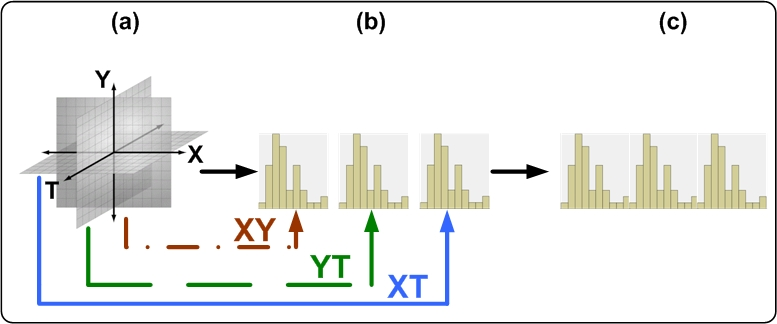
\includegraphics[scale=0.28]{OCPTOP}
\caption{LOCP-TOP Feature Description:(a) Represents feature parameterisation along TOP planes using LOCP operators.(b) Represents the histogram of the LOCP features from each TOP plane.(c) Represents the concatenation of these histograms for use in dynamic texture analysis}
\label{OCPTOP}
\end{figure}

\section{Speaker verification systems}
\label{SpeakerVerificationSystems}
For this system, the method in \cite{Ramos00Thesis} was first used to generate estimates of tracked outer lip contours for all videos. 
The estimated lip contours were then used to localise the mouth-region on a per-frame basis. 
These extracted regions were then used as input information for parameterisation using LOCP-WTOP. 
Each extracted region can be visualised as a cube containing spatiotemporal information. 
The spatiotemporal video cube is divided into 3 or 6 sub-cubes along the T axis and 5 sub-cubes along the Y axis. 
These sub-cubes overlapped each other by 70\%. 
The reason for this overlap was to ensure quantisation of temporally continuous information. 
Additionally, the number of cube partitions values in the T and Y axes respectively enabled us to evaluate the relative performance of the spatial and temporal information in greater detail.  
% These concatenated histograms are then used as input into the speaker verification systems.
For each subcube, we use LOCP-WTOP to extract histograms $\bm{h}_{P,R}^{\beta,j}$ where $j$ represents the subcube index. 
These are then further concatenated to form $\bm{f}^{\alpha,j}$. 
The combined histograms conceptually represent the feature-level fusion of extracted LOCPs in the different planes. 
These histograms are then input into one of two classification engines are described below. 

\textbf{Chi-squared Histogram Matching}: In order to measure the similarity between two input LOCP-WTOP histograms resulting from a probe and an enrolled gallery video, we use a simple, direct measure $Sim_{chi}(\bm{G},\bm{I})$ based on Chi-squared distance between the histograms (with bin index $i$) of two input videos $\bm{G}$ and $\bm{I}$. 
\begin{equation}
\label{MLBP:Chi_sq}
Sim_{\chi}(\bm{G},\bm{I})=-\sum_j \sum_i \frac{(\bm{f}^{\alpha,j}_{G}(i) -\bm{f}^{\alpha,j}_{I}(i))^2}{\bm{f}^{\alpha,j}_{G}(i)+\bm{f}^{\alpha,j}_{I}(i)}
\end{equation}

\textbf{Linear Discriminant Analysis}: In order to extract the discriminative features we project the subcubic histograms, $\bm{f}^{\alpha,j}$, into LDA space as: $\bm{d}^{\alpha,j}=(\bm{W}^{\alpha,j}_{lda})^{T}\bm{f}^{\alpha,j}$. After projection, we perform normalized cross-correlation across all subcubics using two videos $\bm{G}$ and $\bm{I}$ as specified in Equation~\ref{NormCrossCorrelation}.
\begin{equation}
 Sim_{LDA}(\bm{G},\bm{I}) = \sum_{j}\dfrac{(\bm{d}^{\alpha,j}_{G})^{T}\bm{d}^{\alpha,j}_{I}}{\lVert \bm{d}^{\alpha,j}_{G}\rVert\lVert \bm{d}^{\alpha,j}_{I}\rVert}
\label{NormCrossCorrelation}
\end{equation}

\section{Results and Evaluation}
\label{ResultsAndEvaluation}
\subsection{Experimental Set-up}
The mouth-region localisation for the XM2VTS database was set to be 61 by 51 pixels. 
LOCP feature parameters $P$ and $R$ were set to 8 and 3 respectively. 
Additionally, they were set to be the same for all planar configurations. 
The XM2VTSDB \cite{Messer99Xm2vts} database, is a large multi-modal database intended for training and testing multi-modal verification systems. 
It contains synchronised video and speech data along with image sequences that allow multiple views of the face. 
The database consists of digital video of 295 subjects. 
For these experiments, we followed the Configuration I (C1) and Configuration II (C2) of the Lausanne protocol that accompanies this database for speaker verification. 
\subsection{Results}
\paragraph*{TOP Planar Configuration Evaluation}
\begin{table}[htpb!]
\setlength{\tabcolsep}{3pt}
\rowcolors{3}{white}{Lavender}
\resizebox{8.5cm}{!}{
\begin{tabular}{ccccc}
\toprule
\multirow{2}{2cm}{\centering\textbf{TOP Plane}}&\multicolumn{2}{c}{\textbf{Configuration
I}}&\multicolumn{2}{c}{\textbf{Configuration II}}\\
&\textbf{ Eval}&\textbf{Test}&\textbf{Eval}&\textbf{Test}\\
\midrule
XYXTYT&3.17&3.9&4.26&4.43\\ 
XY&3.7&3.7&4.25&4.27\\ 
XT&18.33&19.85&19.73&19.75\\ 
YT&9.05&10.41&11.55&10.73\\ 
XYXT&3.46&3.75&4.72&4.38\\ 
XYYT&\textbf{2.71}&\textbf{2.79}&\textbf{2.98}&\textbf{3.31}\\ 
XTYT&11.7&13.14&13.17&13.62 \\ \hline
\end{tabular}
}
\caption{EER and HTER Performance for LOCP Histograms with Chi-Squared Histogram Matching in \%}
\label{TOPChi}
\end{table}
\begin{table}[htpb!]
\setlength{\tabcolsep}{3pt}
\rowcolors{3}{white}{Lavender}
\resizebox{8.5cm}{!}{
\begin{tabular}{ccccc}
\toprule
\multirow{2}{2cm}{\centering\textbf{TOP Plane}}&\multicolumn{2}{c}{\textbf{Configuration
I}}&\multicolumn{2}{c}{\textbf{Configuration II}}\\
&\textbf{ Eval}&\textbf{Test}&\textbf{Eval}&\textbf{Test}\\
\midrule
\textbf{XYXTYT}&\textbf{0.33}&\textbf{0.65}&\textbf{0.76}&\textbf{0.95}\\ 
XY&1.16&1.04&1.28&1.29\\ 
XT&7.97&8.59&9.06&10.19\\ 
YT&2.8&5.03&4.13&5.38\\ 
XYXT&0.5&0.84&1.29&1.22\\ 
XYYT&0.51&0.82&0.98&0.991\\ 
XTYT&2.01&3.56&2.52&4.22 \\ \hline
\end{tabular}
}
\caption{EER and HTER Performance for LOCP Histograms with Normalised Correlation(with LDA) Histogram Matching in \%}
\label{TOPLDA}
\end{table}
Tables~\ref{TOPChi} and \ref{TOPLDA} show the HTER of the test-set and the EER of the evaluation-set of the various LOCP-TOP histograms with the X2 and NC verification systems respectively. 
% The reference LBP operator results are also included for completeness.
% The ROC curves are shown in Figs~\ref{ROCC1},\ref{ROCC2}. 
The best performances (highlighted in bold) were obtained using XYYT histograms with the chi-squared system for C1 and the XYXTYT histograms with the LDA system for C2. 
The first notable observation is that the performance of the speaker verification engine using NC is significantly better (2 times better in the worst case) than using X2. 
This is unsurprising, NC is performed in the discriminative space(LDA projection) while Chi-squared distance is applied to the raw feature histograms. 
The XY plane outperforms both the temporal planes implying that the appearance differences between clients are more discriminative than their lip dynamics. 
Another interesting observation is that the performance along the XT plane in any configuration degrades the system performance except in LDA space. 
This is because mandibular deformation during speech production primarily manifests itself in the YT direction. 
\paragraph*{Performance of WTOP}
\begin{table}[htpb!]
\centering
\setlength{\tabcolsep}{3pt}
\rowcolors{3}{white}{Lavender}
\resizebox{8.5cm}{!}{
% \scalebox{0.5}{!}{
\begin{tabular}{ccccccccc}
\toprule
\multirow{3}{*}{\centering\textbf{TOP Input}}&\multicolumn{4}{c}{\textbf{Configuration I}}&\multicolumn{4}{c}{\textbf{Configuration II}}\\
&\multicolumn{2}{c}{\textbf{LBP}}&\multicolumn{2}{c}{\textbf{LOCP}}&\multicolumn{2}{c}{\textbf{LBP}}&\multicolumn{2}{c}{\textbf{LOCP}}\\
&\textbf{ Eval}&\textbf{Test}&\textbf{Eval}&\textbf{Test}&\textbf{ Eval}&\textbf{Test}&\textbf{Eval}&\textbf{Test} \\
\midrule
TOP	&3.18	&3.52	&2.99	&3.86	&4.46	&3.60	&4.27	&3.97\\
WTOP, $\sigma=0.1$	&3.32	&3.77	&3.21	&3.69	&4.48	&3.68	&4.23	&3.92\\
WTOP, $\sigma=0.5$	&3.41	&4.03	&3.22	&3.69	&4.71	&3.83	&4.41	&3.97\\
WTOP, $\sigma=1$	&3.36	&3.95	&3.17	&3.59	&4.26	&4.07	&3.99	&3.74\\
WTOP, $\sigma=10$	&3.00	&3.19	&2.51	&3.04	&4.43	&4.11	&4.01	&3.49\\
WTOP, $\sigma=100$	&3.92	&4.28	&3.82	&3.82	&6.51	&5.63	&6.26	&5.8\\
\hline
\end{tabular}
}
\caption{LOCP/LBP-WTOP performance using the Chi-squared system}
\label{WTOPChi}
\end{table}
\begin{table}[htpb!]
\centering
\setlength{\tabcolsep}{3pt}
\rowcolors{3}{white}{Lavender}
\resizebox{8.5cm}{!}{
% \scalebox{0.5}{!}{
\begin{tabular}{ccccccccc}
\toprule
\multirow{3}{*}{\centering\textbf{TOP Input}}&\multicolumn{4}{c}{\textbf{Configuration I}}&\multicolumn{4}{c}{\textbf{Configuration II}}\\
&\multicolumn{2}{c}{\textbf{LBP}}&\multicolumn{2}{c}{\textbf{LOCP}}&\multicolumn{2}{c}{\textbf{LBP}}&\multicolumn{2}{c}{\textbf{LOCP}}\\
&\textbf{ Eval}&\textbf{Test}&\textbf{Eval}&\textbf{Test}&\textbf{ Eval}&\textbf{Test}&\textbf{Eval}&\textbf{Test} \\
\midrule
TOP	&0.87	&1.29	&0.25	&0.36	&1.5	&1.67	&0.99	&0.49\\
WTOP, $\sigma=0.1$	&0.86	&1.64	&0.33	&0.38	&1.3	&1.57	&0.76	&0.5\\
WTOP, $\sigma=0.5$	&0.87	&1.43	&0.33	&0.38	&1.51	&1.53	&0.75	&0.62\\
WTOP, $\sigma=1$	&0.83	&1.75	&0.19	&0.44	&1.53	&1.53	&0.75	&0.62\\
WTOP, $\sigma=10$	&0.84	&1.01	&0.33	&0.09	&\textbf{1.25}	&\textbf{0.96}	&\textbf{0.61}	&\textbf{0.27}\\
WTOP, $\sigma=100$	&0.86	&1.18	&0.33	&0.35	&1.52	&1.23	&0.96	&0.55\\ 
\hline
\end{tabular}
}
\caption{LOCP/LBP-WTOP performance using the Normalised Correlation system}
\label{WTOPLDA}
\end{table}
Tables~\ref{WTOPChi} and \ref{WTOPLDA} show the performance figures for LOCP-WTOP histograms. 
We have also included the results of the LBP-WTOP for reference. 
Note that in these tables, only the best performing TOP configuration i.e. XYXTYT was used.
Various width ($\sigma$) values for the Gaussian windowing function were used. 
A final point to note was the comparison between LOCP and LBP which belong to the same family of ordinal contrast measures. 
The performance of LOCP and LBP in the X2 system were comparable.
However, LOCP outperformed the LBP representation when combined with the NC system.
\paragraph*{Comparison to literature}
The results obtained demonstrated a marked and remarkable improvement on the best performance observed on this database in the literature (HTER=13.35) and indeed the result of the XYXTYT LOCP-TOP histograms using LDA is comparable to the state-of-the-art system performance using multi-modal fusion with audio and face features. 
This is due to the encapsulation of discriminative, dynamic and appearance textures using LOCP-TOP and the implicit intra-model fusion of both genetic and behavioural properties of the observed subject lip-regions. 

\section{Conclusions and Future Work}
\label{Conclusions}
We first presented a thorough review of the current state-of-the-art lip biometric systems. In this paper, we have proposed a novel ordinal contrast measure called LOCP. This has been used in a TOP configuration as input into speaker verification systems using chi-squared histogram distance and LDA respectively. The resulting biometric systems have been used to evaluate the performance of mouth-region biometrics in the XM2VTS database using the standard Lausanne protocols. The application of this novel feature representation has been demonstrated to comprehensively outperform previous feature descriptors encountered in the state-of-the-art. The findings also suggest that there is sufficient discriminative information within the spatiotemporal evolution of the mouth-region during speech production for its use as a primary biometric trait. This can be especially useful in circumstances where auditory information may not be available for fusion. Finally, LOCP histograms are computationally simple compared to the more exotic feature parameterisations encountered in the literature.

\noindent\small{{\bf{Acknowledgments}:} This work is supported by the EU-funded MOBIO project grant IST-214324.}
\bibliography{../Thesis/Bib/BioMetricsBib,../Thesis/Bib/ModellingBib,../Thesis/Bib/SegBib} 
\bibliographystyle{plain}

\end{document}
